\subsubsubsection{Interface Layer}

Figure \ref{fig:impl-il-arch} provides an high level view of
the Interface Layer (IL) components.

\begin{figure}[H]
  \centering
  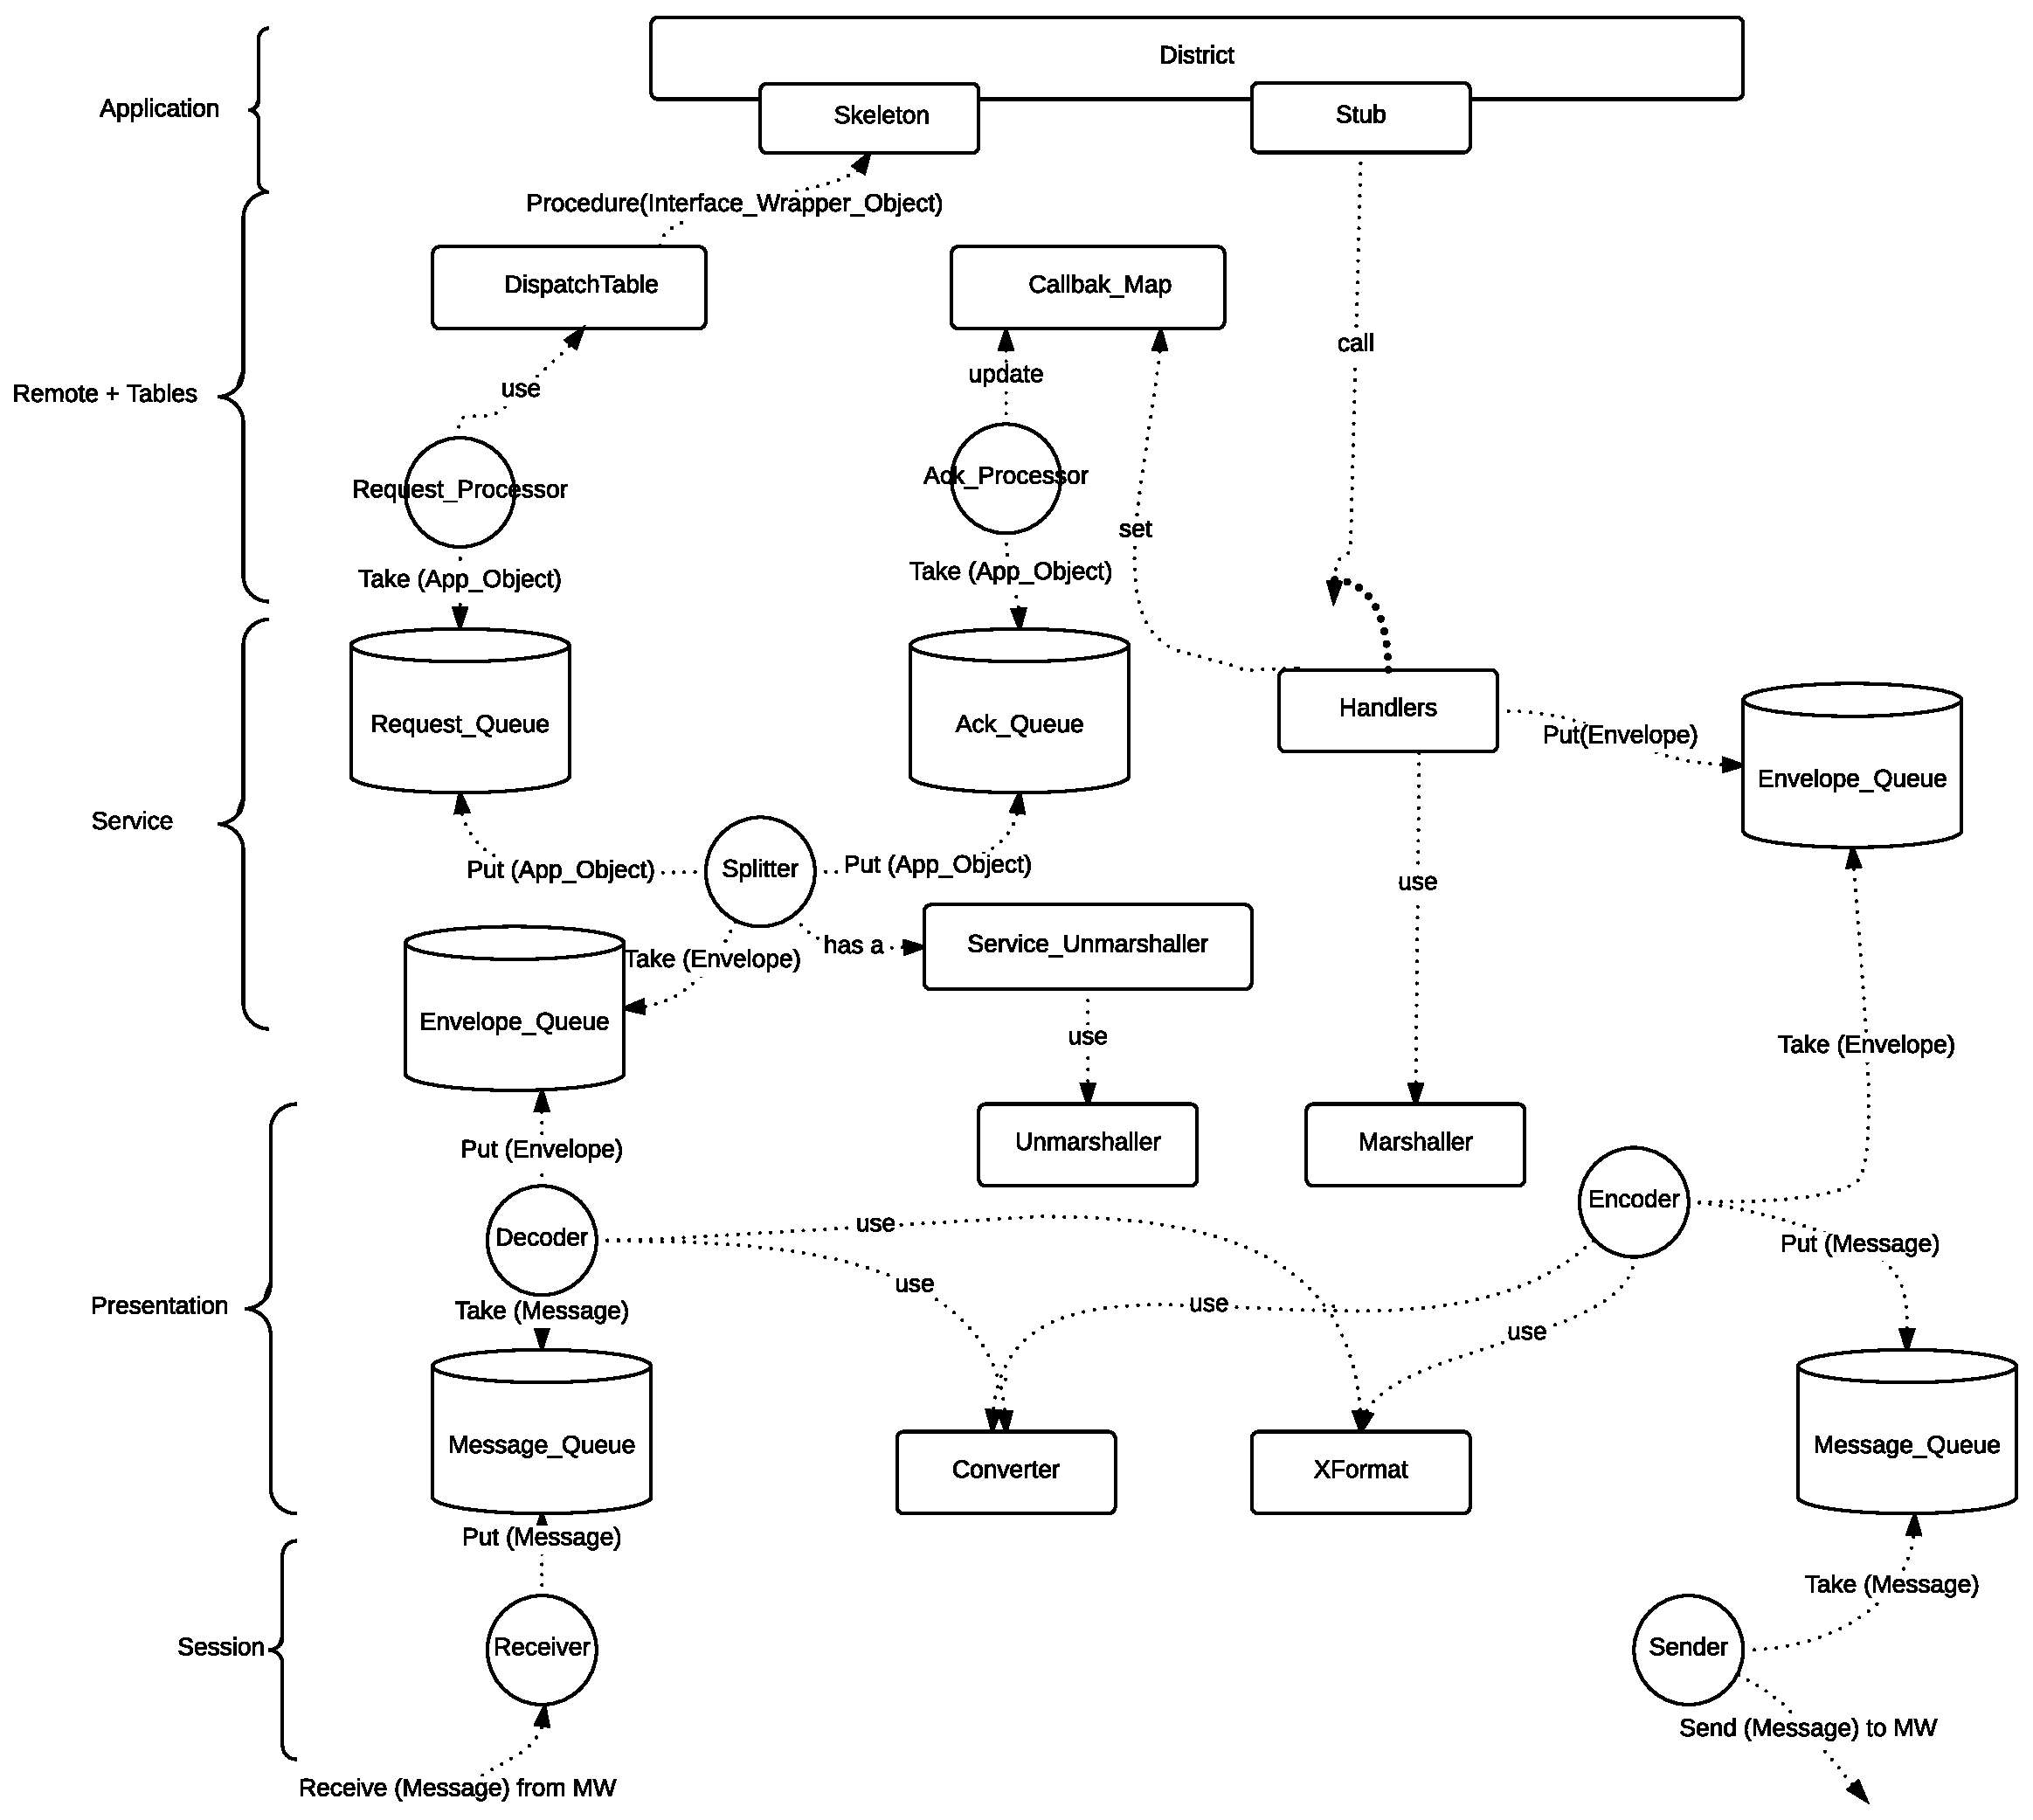
\includegraphics[width=\columnwidth]{images/implementation/il-overall.eps}
  \caption{Interface Layer architecture}
  \label{fig:impl-il-arch}
\end{figure}

IL enables the Application Layer to communicate with other applications
transparently without knowing if they are local or remote. We leverage data
encapsulation by wrapping the application data as the payload of messages while
different sub-layers of IL manipulate different fields of the
message header.
This layered approach has been inspired by the TCP/IP and ISO/OSI models, in
which the layers communicate in two directions:
\begin{itemize}
	\item horizontally - manipulating the same fields of the header;
	\item vertically  - passing the packet to the next
layer, which is charged with different responsibilities.
\end{itemize}
Also, IL is completely asynchronous because each of its sub-layers has its own
thread pool that runs in an event loop consuming messages from its own incoming
queue. For example, the receiver can handle potentially multiple concurrent
requests by delegating each one of them to its worker threads. After a worker has
completed the assigned task it is pushed back on the receiver's local stack,
ready to be reused.


In the following we list the sub-layers which compose IL in
bottom up order:

\begin{itemize}
  \item \textit{Session Layer} --
  handles remote connections through TCP sockets;
  \item \textit{Presentation Layer} --
  handles messages formatting and conversions;
  \item \textit{Service Layer} --
  converts remote requests into procedure calls
  by leveraging a skeleton object.
  Also, it offers the specular service through a stub object plus a pipeline
  of handlers. For each request, the former compose a specific pipeline
  of handlers transparently to the Application Layer.
  The handlers are used to incrementally construct the message by adding
  header fields, wrapping the data into a payload field and finally putting
  the message in the first queue which goes downwards (towards the middleware).
  \item \textit{Remote Layer + Tables} --
  It contains the tables used
  to dispatch the remote calls and the callback map of pending requests.
  A pending request is a synchronous requests which may trigger one of
  the following behaviors:
  \begin{itemize}
  	\item retransmission on timeout;
  	\item a local retry on failure - retry on the local district with
  	the next action which could be a repetition of the last executed action;
  	\item a local clean up on success - remove the retained data from the local
  	district. The message has been successfully sent.
  \end{itemize}
  With pending request we are not reinventing a weakened version
  of TCP retransmission timers as it might seem.
  We have concretely faced network connection errors during the communication
  with the middleware layer. This was caused by occasional failures or network
  problems subsequently fixed by the system itself (e.g. docker swarm). However,
  we prefer to keep these synchronous messages as responsibility of the IL
  for two reasons:
  \begin{itemize}
  	\item it is the layer which has the highest probability of not losing them.
  	Indeed, the communication with the Application Layer happens through
  	local procedure
  	calls. Also, the TCP communication with the middleware layer could lead to
  	lose messages;
  	\item the data wrapped in the messages are too important for the
  	application: a failure
  	or a timeout has to trigger a reaction as soon as possible because
  	the latency introduced in this communication can lead to a significant
  	time drift for the end user (e.g., a set of travellers blocked with
  	apparently no reasons). This could undermine the principle of viewing the
  	whole distributed system as one single unit.
  \end{itemize}
\end{itemize}